\documentclass[english,version-2022-01]{uzl-thesis} %version-2020-11

\UzLThesisSetup{
  Logo-Dateiname        = {Logo_IMI_de.png},
  Verfasst              = {am}{Institut für Medizinische Informatik},
  Titel auf Deutsch     = {MRT-Registration}, 
  Titel auf Englisch    = {MRT-Registration},
  Autor                 = {Jan Meyer},
  Betreuerin            = {Prof. Dr. Mattias Heinrich},
  Mit Unterstützung von = {Ziad Al-Haj Hemidi, Eytan Kats},
  Masterarbeit,
  Studiengang           = {Medizinische Informatik},
  Datum                 = {1. Januar 2025},
  Abstract              = {Something about MRI and registration},
  Zusammenfassung       = {Irgendwas über MRT und Registration},
  Acknowledgements      = {Danke an Mattias, Ziad und Eytan für die gute Betreuung.},
  Numerische Bibliographie %Alphabetische
}


% Designs
%\UzLStyle{computer modern oldschool design}
%\UzLStyle{computer modern scholary design}
%\UzLStyle{pagella basic design}
%\UzLStyle{pagella centered design}
%\UzLStyle{pagella contrast design}
%\UzLStyle{alegrya basic design}
%\UzLStyle{alegrya scholary design}
%\UzLStyle{alegrya stylish design}
\UzLStyle{alegrya modern design}




%%%%%%%%
%
% Now, include the package you need here using \usepackage. 
%
% However, many standard packages are already loaded by the class:
% amsmath, amssymb, amsthm, babel, biblatex, csquotes, etoolbox,
% filecontents, fontspec, geometry, hyperref, tikz (with libraries
% arrows.meta, positioning and shapes), varioref, url 
%
%%%%%%%



% add bibliography
%\addbibresource{Bibliography.bib}
\bibliography{Bibliography.bib}


\begin{document}

%%%%%%%%%%%%%%%%%%%%%%%%%
%%%%%  Introduction %%%%%
%%%%%%%%%%%%%%%%%%%%%%%%%

\chapter{Introduction}
Introduction of stuff.

\section{Contributions of the Thesis}
We implemented stuff.

\section{Related Work}
There are many papers on image registration in general, however in the context of medical image registration with deep learning their number is reduced due to the specialized nature of the subject at hand. Yet, there are a couple of papers that give a good overview of the topic.
%like \emph{Deep learning in medical image registration}
They give a brief overview of registration methods, basics of deep learning with already existing networks for image registration as well as covering potential applications and challenges~\cite{Chen2020,Haskins2020,Fu2020,Zou2022,Chen2023}.


\section{Structure of the Thesis}
This Thesis contains a lot of stuff in different chapters.

%%%%%%%%%%%%%%%%%%%%%%%
%%%%%%%  Basics %%%%%%%
%%%%%%%%%%%%%%%%%%%%%%%

\chapter{Basics}
In this chapter the basics of the thesis are explained.

\section{Magnetic Particle Imaging}
Here MRI is described. % TODO: define abbreviations for CT and MRI here!!

\section{Image Registration}
Image registration is a challenging, yet important task for image processing. It can be described as the process of transforming different
image datasets into one coordinate system with matched imaging contents~\cite{Haskins2020}. In the medical field this can be used for clinical applications such as disease diagnosis and monitoring, image-guided treatment delivery, and post-operative assessment. Medical image registration is typically used to preprocess data for tasks like object detection (for e.g. tumor growth monitoring) and segmentation (for e.g. organ atlas creation) where variation in spatial resolution is common between modalities like CT and MRI and patients. Thus the performance of these methods is dependent on the quality of image registration~\cite{Chen2020}. \\
Medical image registration was often done manually by clinicians, however, registration tasks are often challenging and the quality of manual alignments is dependent on the expertise of the user. These manual registrations are thus not only time consuming, but also hardly reproducible leading to high interobserver-variability. The need for automatic registration is very much apparent, but this task remained hard to solve for a long time, requiring a lot of computational power and time for computer algorithms to solve the problem. While neural networks also require a lot of computational power and time to train, they promise fast execution after training. With the rise of deep learning these network gained popularity and now pose a real alternative to conventional algorithms and manual registration~\cite{Haskins2020}. We will discuss these new approaches in the next section, but first we need to formally define our problem.\\
In pair-wise image registration two images ($F$ and $M$) are to be aligned, with $F$ denoting the fixed and $M$ the moving image. T is the desired spatial transformation that aligns the two images. This can be posed as an optimization problem:
\begin{equation}
	T' = \arg\max S(F, T(M)),
\end{equation}
with $T'$ being the best transformation that maximizes the similarity $S$ between the two images. This process is done iteratively improving estimates for the desired T, such that the defined similarity in the cost function is maximized~\cite{Chen2020}.\\
Transformations can be categorized as rigid, affine, and deformable. A rigid transformation consists of rotation and translation; an affine transformation
includes translations, rotations, scaling, and sheering; the two kinds of transformations are described as a 2D single matrix. Unlike rigid and affine transformation, deformable transformation is a high-dimension problem that we need to formulate by a 3D matrix for 2D deformable registration i.e., a so-called deformation field. While rigid and affine registration algorithms have already achieved good performance in many applications, deformable registration is still a challenging task due to its intrinsic complexity, particularly when the deformation is large. However, these are also the transformations most likely encountered in clinical practice as it can be utilized to fuse information from different modalities such as MRI and CT~\cite{Zou2022}. Additionally, deformable image registration can also be
utilized for various computer-assisted interventions like biopsy~\cite{Tam2016} and (MRI-guided) radiotherapy~\cite{Chen2017, Rigaud2019}. \\
Intuitively, deformable image registration is an ill-posed problem, making it fundamentally different from other computer vision tasks such as object localization, segmentation or classification. Given two images, deformable image registration aims to find a spatial transformation that warps the moving image to match the fixed image as closely as possible. However, there is no ground-truth available for the desired deformation field and without enforcing any constraints on the properties of the spatial transformation, the resulting cost function is ill-conditioned and highly non-convex. In order to address the latter and ensure tractability, all image registration algorithms regularize the estimated deformation field, based on some prior assumptions on the properties of the underlying unknown deformation~\cite{Chen2020}.\\
Many methods have been proposed for medical image registration to deal with the complex challenges of this task. Popular conventional registration methods include optical flow~\cite{Yang2008}, demons~\cite{Vercauteren2009} and many more. However, most of these still lack accuracy and computation speed, which makes newer deep learning approaches all the more interesting~\cite{Fu2020}.

\section{Deep Learning Basics}
Deep Learning has seen a rise in popularity in the last year in various fields including image registration. \\
Some basic stuff about network training, testing and different architectures that are relevant for the later Chapters.

\subsection{CNNs}
CNNs are an important class of neural networks, mainly for image processing.

\subsection{U-Net}
The U-Net~\cite{U-Net} architecture is typically used for segmentation, but can also be used for image registration tasks.

\section{Deep Learning for Image Registration}
Which different kinds of deep learning approaches are there for image registration.

\subsection{Supervised Registration}
Supervised Registration describes training a network with a ground truth displacement field that is either real or synthetic. Thus the loss can easily be calculated as the difference in the displacement fields of the network and ground truth. These methods have achieved notable results with real displacement fields as supervision. However, this is limited by the size and the diversity of the dataset. The real displacement field are also often calculated by conventional algorithms, which might limit their effectiveness for difficult problems. Fully supervised methods are widely studied and have notable results, but the generation of real or synthetic displacement fields is hard, and these displacements fields might be different from the real ground truth, which can impact the accuracy and efficiency of these kinds of methods~\cite{Zou2022}.

\subsection{Unsupervised Registration}
As the preparation of the ground truth displacement field for supervised methods is inconvenient, limitations in generalizing results in different domains and various registration tasks are inevitable. Thus, unsupervised registration has a more convenient training process with paired images as inputs, but without a ground truth. Generally, unsupervised learning consists of similarity-based and GAN-based methods~\cite{Zou2022}.


%%%%%%%%%%%%%%%%%%%%%%%%
%%%%%  Methodology %%%%%
%%%%%%%%%%%%%%%%%%%%%%%%

\chapter{Methodology}
In this chapter the main part of the actual work is discussed.

\section{Data}
Describe the data used for evaluation.

\section{Network Architecture}
Describe the network being used.

\subsection{Fourier-Net}
The \emph{Fourier-Net}  is new approach that aims to learn a low-dimensional representation of the displacement field in a band-limited Fourier domain instead of the full field in the spatial domain. This band-limited representation is then decoded by our devised model-driven decoder to the dense, full-resolution displacement field in the spatial domain. These changes allow for fewer parameters and computational operations, resulting in faster inference speeds~\cite{Fourier-Net}. The architecture is based on the U-Net~\cite{U-Net}, like most deep registration approaches, but replaces the expansive path with a parameter-free model-driven decoder as mentioned before.\\
The encoder of \emph{Fourier-Net} consists of a CNN that is based on the networks in~\cite{Zhang2018,Mok2020} and a DFT that converts the displacement field from the spatial domain into the Fourier domain, thus band-limiting the field. From there the band-limiting representation is padded with zeros to the full resolution of the original displacement field. The field is then recovered by using the inverse DFT (iDFT) to convert it back into the spatial domain. This displacement field is then used to warp the moving image into the fixed image. Optionally squaring and scaling layers can also be added before warping the image to improve the reconstruction of the displacement field. A diagram of this can be seen in Figure~\ref{fig:Fourier-Net}.


\begin{figure}[htpb]
	\centering
	\graphicspath{{images/}{\main/images/}}
	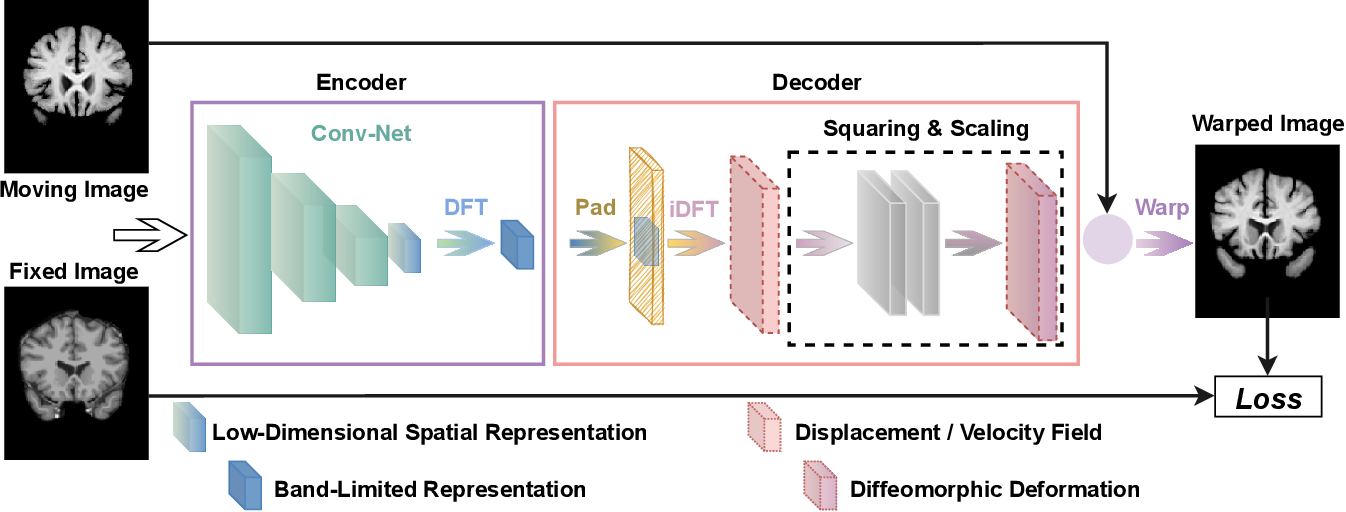
\includegraphics[width=\linewidth]{ArchitectureFourier-Net.png} 
	\caption{Architecture of Fourier-Net taken from~\cite{Fourier-Net}}
	\label{fig:Fourier-Net}
\end{figure}


\subsection{Fourier Net+}
Here goes the explanation for the Fourier Net+.

\section{Evaluation}
Describe the evaluation methods being used.


%%%%%%%%%%%%%%%%%%%%%%%%%%%%
%% Results and Discussion %%
%%%%%%%%%%%%%%%%%%%%%%%%%%%%

\chapter{Results and Discussion}
Here go the results with the discussion.


%%%%%%%%%%%%%%%%%%%%%%%
%%%%%  Conclusion %%%%%
%%%%%%%%%%%%%%%%%%%%%%%

\chapter{Conclusion}
Summery of all stuff...

\end{document}